\documentclass[11pt]{article}
\usepackage[margin=1in]{geometry}
\usepackage{amsmath,amssymb,amsthm,mathtools,bm}
\usepackage{graphicx,booktabs,subcaption}
\usepackage[hidelinks]{hyperref}
\usepackage{enumitem}
\allowdisplaybreaks

\newtheorem{proposition}{Proposition}[section]
\newtheorem{theorem}[proposition]{Theorem}
\newtheorem{remark}[proposition]{Remark}
\newtheorem{definition}[proposition]{Definition}

\newcommand{\R}{\mathbb{R}}
\newcommand{\E}{\mathbb{E}}
\newcommand{\Var}{\operatorname{Var}}
\newcommand{\Cov}{\operatorname{Cov}}
\newcommand{\diag}{\operatorname{diag}}
\newcommand{\Id}{I}
\newcommand{\trans}{\mathsf{T}}
\newcommand{\Ncal}{\mathcal{N}}
\newcommand{\norm}[1]{\left\lVert #1 \right\rVert}
\newcommand{\abs}[1]{\left| #1 \right|}

\title{Deterministic Limit of AR(1) Diffusion\\[2mm]
\large Global coupling without innovation noise}
\author{}
\date{}

\begin{document}
\maketitle

\begin{abstract}
We remove the AR(1) innovation noise and keep only a random initial state. The recursion becomes
\[
 a_{k+1}=\alpha a_k,
 \qquad
 a_k=\alpha^k A_0,
 \qquad
 A_0\sim\Ncal(\mu_0,\sigma_0^2).
\]
The clean trajectory is then supported on the one-dimensional curve $vA_0$. Here
\[
 v=(1,\alpha,\dots,\alpha^K)^\trans.
\]
Its covariance is rank one,
\[
\Sigma_0^{\mathrm{det}}=\sigma_0^2 vv^\trans,
\]
so there is no ordinary precision matrix at $t=0$. After Ornstein--Uhlenbeck corruption,
\[
\Sigma_t^{\mathrm{det}}=e^{-2t}\sigma_0^2 vv^\trans+(1-e^{-2t})\Id,
\]
and the inverse can be computed exactly by solving a rank-one linear system. The result is
\[
Q_t^{\mathrm{det}}=
\frac{1}{\Delta_t}\Id-
\frac{e^{-2t}\sigma_0^2}{\Delta_t\bigl(\Delta_t+e^{-2t}\sigma_0^2\norm{v}^2\bigr)}vv^\trans,
\qquad
\Delta_t=1-e^{-2t}.
\]
Thus every off-diagonal entry is nonzero for every $t>0$. The score of each coordinate depends on a single global weighted sum of all coordinates. This shows that loss of locality does not require stochastic innovations: propagation of one shared latent variable already creates global coupling.
\end{abstract}

\section{Setup: removing the innovation noise}
Start from the usual AR(1) recursion
\[
 a_{k+1}=\alpha a_k+\eta_k.
\]
The deterministic limit is obtained by setting $\eta_k\equiv 0$, so
\begin{equation}\label{eq:det_rec}
 a_{k+1}=\alpha a_k,
 \qquad
 a_k=\alpha^k A_0,
 \qquad
 A_0\sim\Ncal(\mu_0,\sigma_0^2).
\end{equation}
Collect the trajectory into the vector
\[
 a=(a_0,a_1,\dots,a_K)^\trans\in\R^N,
 \qquad N=K+1,
\]
and define
\begin{equation}\label{eq:v_def}
 v:=(1,\alpha,\alpha^2,\dots,\alpha^K)^\trans.
\end{equation}
Then the whole trajectory is simply
\begin{equation}\label{eq:a_vA0}
 a= v A_0.
\end{equation}
This is a local recursion in time, but probabilistically it is a single latent variable replicated through the deterministic propagator $v$.

\section{Clean covariance: rank one and globally correlated}
The mean is
\[
 \mu_a:=\E[a]=\mu_0 v.
\]
Subtracting the mean from \eqref{eq:a_vA0},
\[
 a-\mu_a=v(A_0-\mu_0).
\]
Therefore
\begin{equation}\label{eq:sigma0_det}
\Sigma_0^{\mathrm{det}}
:=
\Cov(a)
=
\sigma_0^2 vv^\trans.
\end{equation}
Entrywise,
\begin{equation}\label{eq:sigma0_det_entries}
(\Sigma_0^{\mathrm{det}})_{ij}=\sigma_0^2\alpha^{i+j},
\qquad 0\le i,j\le K.
\end{equation}
Every pair of coordinates is marginally correlated. The dependence pattern is not a function of distance $\abs{i-j}$, but of the shared latent direction $v$.

\begin{proposition}[Rank-one structure]\label{prop:rankone}
The clean deterministic covariance has rank one. Its only nonzero eigenvalue is
\begin{equation}\label{eq:only_eig}
\lambda_{\star}=\sigma_0^2\norm{v}^2,
\qquad
\norm{v}^2=\sum_{k=0}^{K}\alpha^{2k}
=
\begin{cases}
\dfrac{1-\alpha^{2N}}{1-\alpha^2}, & \alpha^2\ne 1,\\[2mm]
N, & \alpha^2=1.
\end{cases}
\end{equation}
\end{proposition}

\begin{proof}
For any vector $x$,
\[
\Sigma_0^{\mathrm{det}}x=\sigma_0^2 v(v^\trans x).
\]
So the image of $\Sigma_0^{\mathrm{det}}$ is the one-dimensional span of $v$, hence the rank is one. Taking $x=v$ gives
\[
\Sigma_0^{\mathrm{det}}v=\sigma_0^2\norm{v}^2v,
\]
so $v$ is an eigenvector with eigenvalue $\lambda_\star=\sigma_0^2\norm{v}^2$. Every vector orthogonal to $v$ is sent to zero.
\end{proof}

Because the clean law lives on a one-dimensional subspace, it has no ordinary density on $\R^N$ and therefore no honest precision matrix $Q_0=(\Sigma_0^{\mathrm{det}})^{-1}$. If one wants an algebraic substitute, the Moore--Penrose pseudoinverse is
\begin{equation}\label{eq:pseudoinverse}
(\Sigma_0^{\mathrm{det}})^+
=
\frac{1}{\sigma_0^2\norm{v}^4}vv^\trans,
\end{equation}
which is already dense. But this pseudoinverse is not a Gaussian conditional-independence object; the clean measure is singular.

\section{Adding diffusion noise restores invertibility}
Let $z\sim\Ncal(0,\Id_N)$ be independent of $a$ and define the noisy observation
\begin{equation}\label{eq:xt}
 x=e^{-t}a+\sqrt{\Delta_t}\,z,
 \qquad
 \Delta_t:=1-e^{-2t},
 \qquad
 \beta_t:=e^{-2t}.
\end{equation}
Then
\[
 \mu_t:=\E[x]=e^{-t}\mu_a=e^{-t}\mu_0 v,
\]
and, using \eqref{eq:sigma0_det},
\begin{equation}\label{eq:sigmat_det}
\Sigma_t^{\mathrm{det}}
=
\beta_t\sigma_0^2 vv^\trans+\Delta_t\Id.
\end{equation}
Now the matrix is strictly positive definite for every $t>0$, so an ordinary inverse exists.

\subsection{Derivation of the inverse from scratch}
We solve the linear system
\[
(\Delta_t\Id+\beta_t\sigma_0^2 vv^\trans)u=b
\]
for arbitrary $b\in\R^N$. Because the perturbation is rank one, it is natural to seek $u$ in the form
\begin{equation}\label{eq:ansatz}
 u=\frac{1}{\Delta_t}b+\lambda v
\end{equation}
for some scalar $\lambda$. Substitute \eqref{eq:ansatz} into the equation:
\begin{align*}
(\Delta_t\Id+\beta_t\sigma_0^2 vv^\trans)u
&=
\Delta_t\left(\frac{1}{\Delta_t}b+\lambda v\right)
+
\beta_t\sigma_0^2 vv^\trans\left(\frac{1}{\Delta_t}b+\lambda v\right) \\
&=
 b+
 \lambda\Delta_t v+
 \frac{\beta_t\sigma_0^2}{\Delta_t}v(v^\trans b)+
 \beta_t\sigma_0^2\lambda\norm{v}^2v.
\end{align*}
For this to equal $b$, the coefficient of $v$ must vanish:
\[
\lambda\Delta_t+
\frac{\beta_t\sigma_0^2}{\Delta_t}(v^\trans b)+
\beta_t\sigma_0^2\lambda\norm{v}^2=0.
\]
Hence
\begin{equation}\label{eq:lambda_det}
\lambda
=
-
\frac{\beta_t\sigma_0^2}{\Delta_t\bigl(\Delta_t+\beta_t\sigma_0^2\norm{v}^2\bigr)}(v^\trans b).
\end{equation}
Substitute \eqref{eq:lambda_det} back into \eqref{eq:ansatz}:
\[
 u=
 \frac{1}{\Delta_t}b-
 \frac{\beta_t\sigma_0^2}{\Delta_t\bigl(\Delta_t+\beta_t\sigma_0^2\norm{v}^2\bigr)}v(v^\trans b).
\]
Because this holds for every right-hand side $b$, we have proved the inverse formula.

\begin{theorem}[Exact deterministic noisy precision]\label{thm:qdet}
For every $t>0$,
\begin{equation}\label{eq:qdet}
Q_t^{\mathrm{det}}
:=
\bigl(\Sigma_t^{\mathrm{det}}\bigr)^{-1}
=
\frac{1}{\Delta_t}\Id-
\frac{\beta_t\sigma_0^2}{\Delta_t\bigl(\Delta_t+\beta_t\sigma_0^2\norm{v}^2\bigr)}vv^\trans.
\end{equation}
Equivalently, for $i\ne j$,
\begin{equation}\label{eq:qdet_offdiag}
(Q_t^{\mathrm{det}})_{ij}
=
-
\frac{\beta_t\sigma_0^2}{\Delta_t\bigl(\Delta_t+\beta_t\sigma_0^2\norm{v}^2\bigr)}\alpha^{i+j}.
\end{equation}
So every off-diagonal entry is nonzero whenever $\alpha\ne 0$.
\end{theorem}

The deterministic benchmark therefore has a very different dense pattern from the Gaussian AR(1) benchmark. In the Gaussian model, the long-range entries are created by inverting a matrix with local structure and typically decay with distance $\abs{i-j}$. In the deterministic model, the off-diagonal part is the separable rank-one matrix $vv^\trans$.

\section{Score: every coordinate sees a global weighted sum}
Because $x$ is Gaussian for every $t>0$, the score is affine:
\begin{equation}\label{eq:score_det}
S^{\mathrm{det}}(x,t)=\nabla_x\log p_t(x)=-Q_t^{\mathrm{det}}(x-\mu_t).
\end{equation}
Insert \eqref{eq:qdet}. If we define
\begin{equation}\label{eq:ct_def}
 c_t:=\frac{\beta_t\sigma_0^2}{\Delta_t\bigl(\Delta_t+\beta_t\sigma_0^2\norm{v}^2\bigr)},
\end{equation}
then
\begin{equation}\label{eq:score_det_expand}
S^{\mathrm{det}}(x,t)
=
-
\frac{x-\mu_t}{\Delta_t}
+
 c_t\,v\,v^\trans(x-\mu_t).
\end{equation}
The $k$th component is therefore
\begin{equation}\label{eq:score_det_component}
S_k^{\mathrm{det}}(x,t)
=
-
\frac{x_k-\mu_{t,k}}{\Delta_t}
+
 c_t\alpha^k\sum_{j=0}^{K}\alpha^j(x_j-\mu_{t,j}).
\end{equation}
This is the key structural fact: \emph{every score component depends on the same global scalar statistic}
\[
\sum_{j=0}^{K}\alpha^j(x_j-\mu_{t,j}).
\]
The coupling is global even though the underlying recursion \eqref{eq:det_rec} is one-step local.

\section{Comparison with the stochastic Gaussian AR(1) model}
\subsection{What disappears when $\sigma_\eta^2\to 0$?}
In the stochastic Gaussian AR(1) model,
\[
 a_{k+1}=\alpha a_k+\eta_k,
 \qquad
 \eta_k\sim\Ncal(0,\sigma_\eta^2),
\]
the clean precision is tridiagonal:
\[
Q_0^{\mathrm{sto}}=
\begin{pmatrix}
\sigma_0^{-2}+\alpha^2\sigma_\eta^{-2} & -\alpha\sigma_\eta^{-2} & & \\
-\alpha\sigma_\eta^{-2} & (1+\alpha^2)\sigma_\eta^{-2} & \ddots & \\
& \ddots & \ddots & -\alpha\sigma_\eta^{-2} \\
& & -\alpha\sigma_\eta^{-2} & \sigma_\eta^{-2}
\end{pmatrix}.
\]
As $\sigma_\eta^2\downarrow 0$, these entries blow up: the quadratic form enforces the hard constraints $a_{k+1}=\alpha a_k$. In covariance language the full-rank Gaussian law collapses onto the rank-one deterministic manifold.

For any fixed $t>0$, however, the noisy covariance stays invertible:
\[
\Sigma_t^{\mathrm{sto}}(\sigma_\eta^2)=e^{-2t}\Sigma_0^{\mathrm{sto}}(\sigma_\eta^2)+\Delta_t\Id.
\]
Since $\Sigma_0^{\mathrm{sto}}(\sigma_\eta^2)\to\sigma_0^2 vv^\trans$ entrywise as $\sigma_\eta^2\to 0$, we immediately obtain
\begin{equation}\label{eq:conv_qt}
\Sigma_t^{\mathrm{sto}}(\sigma_\eta^2)\to\Sigma_t^{\mathrm{det}},
\qquad
Q_t^{\mathrm{sto}}(\sigma_\eta^2)\to Q_t^{\mathrm{det}}.
\end{equation}
So the deterministic benchmark is not a separate curiosity; it is the regularized small-noise limit of the Gaussian AR(1) model.

\subsection{What is the conceptual difference?}
The stochastic Gaussian benchmark and the deterministic benchmark separate two notions that are easy to confuse:
\begin{enumerate}[leftmargin=1.5em]
\item \textbf{Local dynamics.} Both models are generated by a one-step recursion.
\item \textbf{Probabilistic Markov locality.} Only the full-rank Gaussian model has a clean tridiagonal precision encoding conditional independence.
\item \textbf{Global latent coupling.} In the deterministic limit all coordinates are functions of the same scalar $A_0$, so diffusion reveals a dense rank-one interaction pattern.
\end{enumerate}
Thus randomness is not what creates global coupling. Propagation through a shared latent variable already does it.

\section{Numerical illustrations}
All figures were generated by the reproducible script \texttt{code/generate\_figures.py}. We used $\alpha=0.9$, $\sigma_0^2=1$, and $N=60$.

\begin{figure}[ht!]
\centering
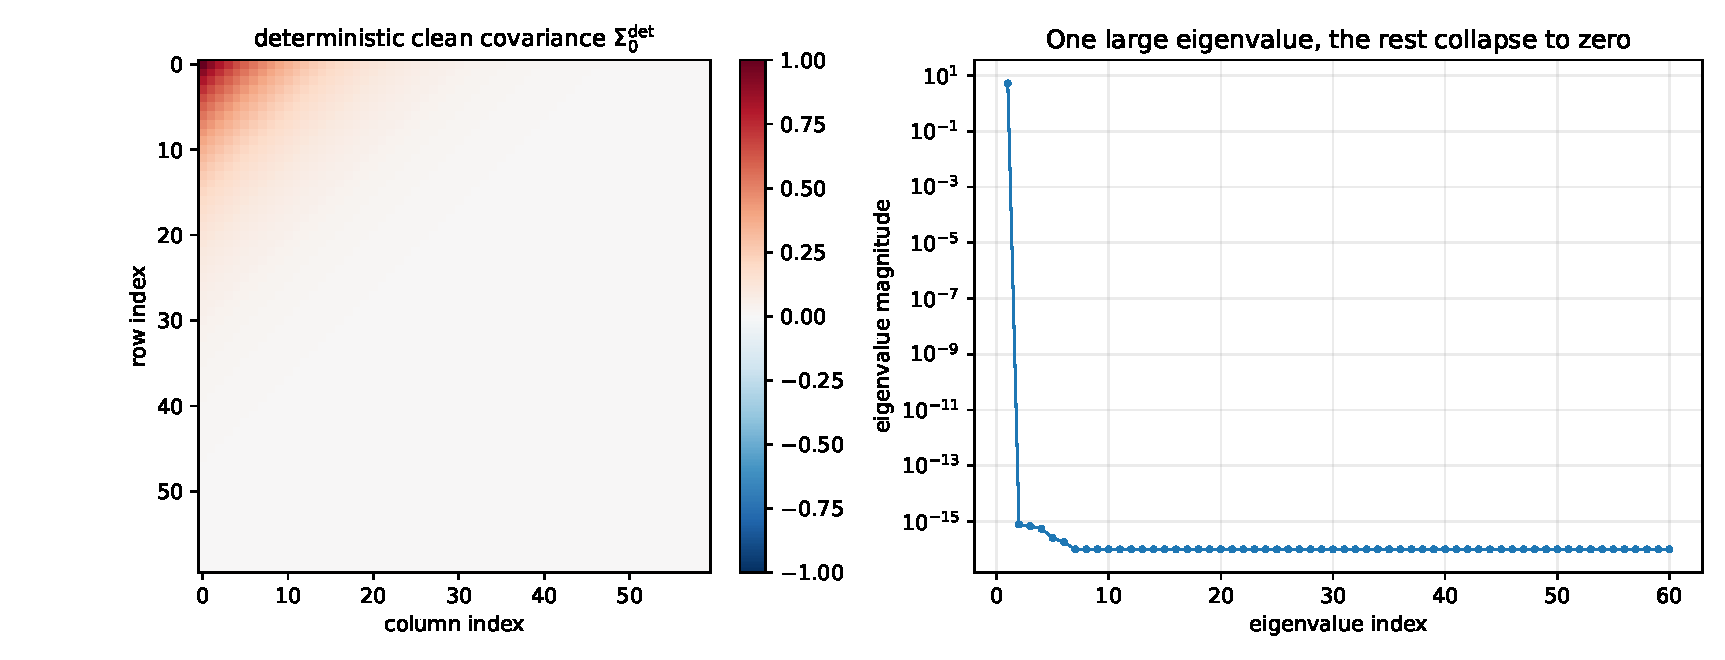
\includegraphics[width=.92\textwidth]{figures/fig01_rankone_covariance.pdf}
\caption{Deterministic clean covariance. Left: heatmap of $\Sigma_0^{\mathrm{det}}=\sigma_0^2vv^\trans$, which is dense although rank one. Right: eigenvalues on a log scale, showing one nonzero mode and numerical zeros for the rest.}
\end{figure}

\begin{figure}[ht!]
\centering
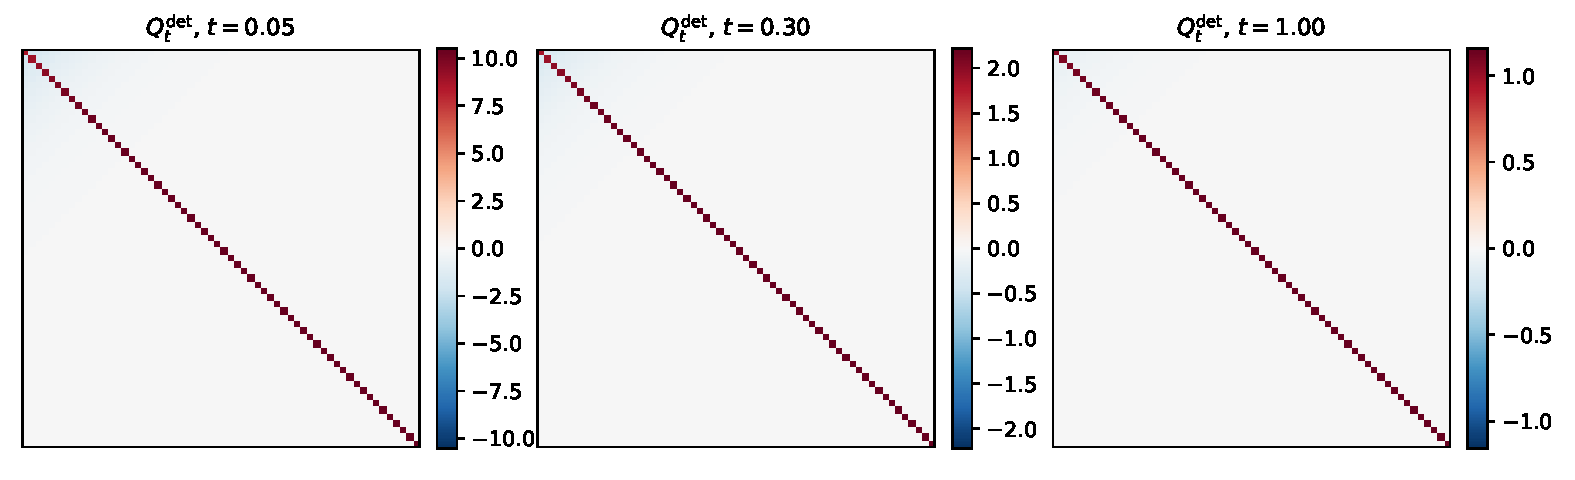
\includegraphics[width=.95\textwidth]{figures/fig02_deterministic_qt.pdf}
\caption{Heatmaps of $Q_t^{\mathrm{det}}$ at three diffusion times. The matrix is always diagonal minus a dense rank-one correction. No notion of nearest-neighbor sparsity survives.}
\end{figure}

\begin{figure}[ht!]
\centering
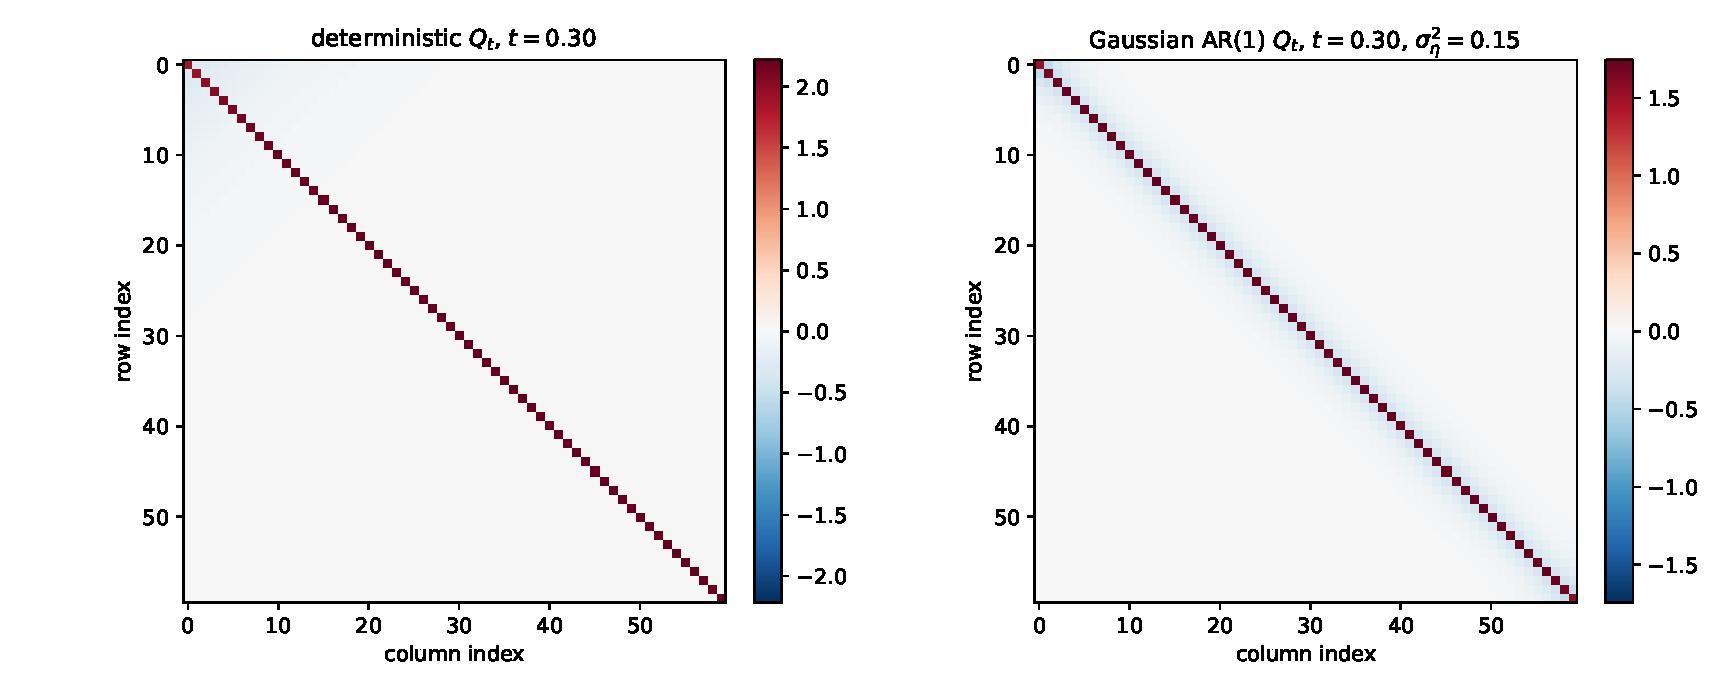
\includegraphics[width=.95\textwidth]{figures/fig03_compare_gaussian_vs_det.pdf}
\caption{Deterministic versus stochastic Gaussian AR(1) at the same diffusion time. The deterministic pattern is globally dense and strongly aligned with the latent direction $v$. The stochastic Gaussian pattern reflects Markov fill-in from an originally tridiagonal precision.}
\end{figure}

\begin{figure}[ht!]
\centering
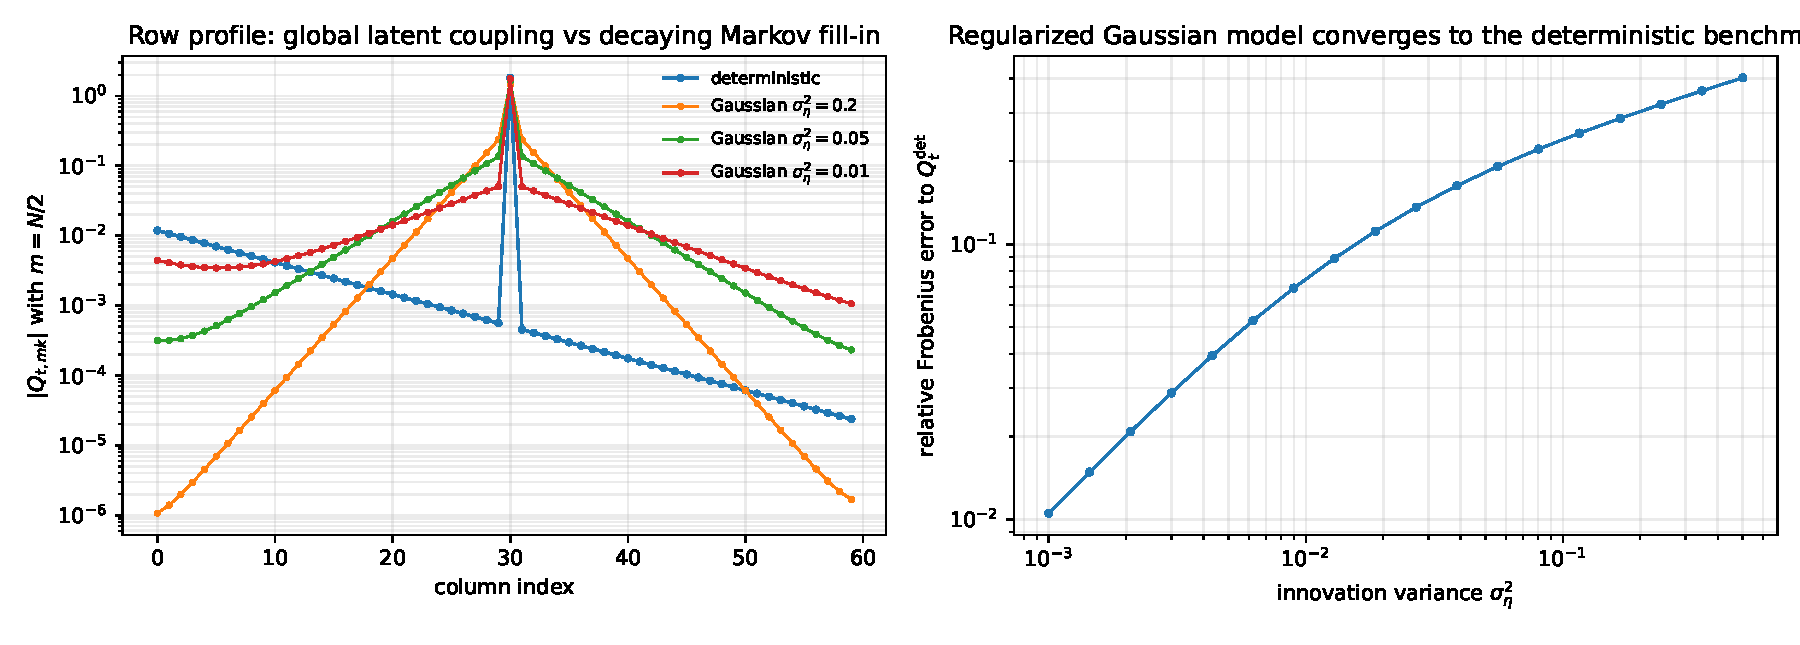
\includegraphics[width=.98\textwidth]{figures/fig04_limit_convergence.pdf}
\caption{Left: a row profile of the precision. The deterministic benchmark couples one row to all columns through the shared latent direction. The Gaussian model has a different profile, but approaches the deterministic one as the innovation variance decreases. Right: the regularized Gaussian precision converges to $Q_t^{\mathrm{det}}$ as $\sigma_\eta^2\to 0$, confirming \eqref{eq:conv_qt}.}
\end{figure}

The figures support four concrete statements:
\begin{enumerate}[leftmargin=1.5em]
\item The clean deterministic covariance is globally correlated even before diffusion.
\item The regularized precision for $t>0$ is dense with a rank-one off-diagonal pattern.
\item This density does not come from stochastic innovations; it comes from the shared latent coordinate $A_0$.
\item The deterministic benchmark is the small-noise limit of the Gaussian AR(1) benchmark at any fixed $t>0$.
\end{enumerate}

\section{Takeaway}
The deterministic limit isolates propagation from randomness. Once the innovations are removed, the trajectory becomes
\[
(a_0,a_1,\dots,a_K)=A_0(1,\alpha,\dots,\alpha^K),
\]
so all coordinates inherit the same latent scalar. The clean covariance collapses to rank one and ceases to admit a full-dimensional precision. After any positive diffusion time, the covariance becomes invertible and its inverse is explicit:
\[
Q_t^{\mathrm{det}}=\frac{1}{\Delta_t}\Id-c_t vv^\trans.
\]
This matrix is dense, not because of Markov noise, but because of deterministic propagation through a shared latent mode. In this sense, the deterministic study cleanly separates two effects:
\[
\text{Markovianity }\neq\text{ global coupling}.
\]
The Gaussian AR(1) model has local conditional structure. The deterministic limit has global latent coupling. Diffusion regularizes both, but the two mechanisms are different.

\end{document}
